\chapter{Net Topo}
\label{cap:proposta}

A contenção de rede e a latência de comunicação são dois fatores ligados à topologia de rede que afetam diretamente o desempenho de uma aplicação paralela e distribuída.
Estes dois fatores podem ser reduzidos com uma distribuição de carga que aloque tarefas que se comuniquem próximas uma da outra~\cite{bhatele-encyclopedia}.
Para saber o quão próximo um PE está de outro e realizar uma alocação eficiente, é preciso obter informações sobre a topologia da rede sendo utilizada.
Ferramentas para descobrimento e uso de informações de topologia existem, mas têm suas limitações.

A ferramenta \hwloc realiza o descobrimento e armazenamento de topologias de máquina, oferecendo um detalhamento profundo de qualquer informação da máquina, mas sem ter qualquer informação inter-máquina.
O projeto \netloc pretende estender o \hwloc adquirindo informações completas da camada de rede, porém está em desenvolvimento e, justamente por procurar um conjunto de informações grande, se torna caro em inicialização e em espaço de memória.
O \textit{runtime} \charm possui uma série de maneiras para utilizar uma topologia de rede, mas estas são enquadradas em alguns tipos de topologias pré-definidas, gerando algumas imprecisões.

Neste capítulo é abordado a Net Topo, uma abstração da topologia de rede criada neste trabalho que visa auxiliar escalonadores e balanceadores de carga cientes de topologia. 
Os objetivos da abstração são abordados na Seção~\ref{sec:net_objetivos}.
A Seção~\ref{sec:estruturas} apresenta as estruturas cogitadas e utilizadas na abstração.
Por último, as funcionalidades da abstração são descritas na Seção~\ref{sec:func}.

\section{Objetivos da Net Topo}
\label{sec:net_objetivos}

O principal objetivo da Net Topo é auxiliar na alocação e distribuição de carga fornecendo informações de uma topologia de rede.
Para que a abstração possa ser utilizada independente da topologia de um sistema, sua representação deve ser flexível e genérica, podendo comportar tipos diferentes de topologias sem perder funcionalidades.
Com isso, a abstração pode ser utilizada em escalonadores e balanceadores independentemente do sistema em que estejam.

O principal uso das informações de topologia para um escalonador ou balanceador de carga é indicar a proximidade entre tarefas, visando a redução de latência e contenção.
Para suprir esta informação, a abstração deve poder indicar a proximidade entre dois PEs na rede e suprir informações de distância como \hops ou latência.

Para acelerar o desenvolvimento e auxiliar escalonadores e balanceadores de carga, é importante que a abstração ofereça métodos úteis e não gere um sobrecusto que degrade o desempenho da aplicação.
Em outras palavras, a Net Topo não pode retardar demasiadamente o processo de distribuição de carga.

Um outro objetivo da abstração é oferecer persistência de informação entre execuções no mesmo sistema, seguindo a ideia do \hwloc de arquivar uma topologia. 
Esse arquivamento permite uma importação posterior das informações de topologia sem passar novamente por um processo de descobrimento, reduzindo o sobrecusto de inicialização da estrutura~\cite{broquedis:hwloc}.
Outro benefício é que o arquivo pode ser repassado para outras máquinas que tenham a mesma topologia de rede, para que não tenham que realizar o descobrimento da topologia.

A plataforma \charm oferece suporte para balanceadores de carga e oferece uma estrutura que facilita o desenvolvimento de um balanceador de carga. 
Um último objetivo da Net Topo é a integração com o módulo de balanceamento de carga do \charm.
Acoplar a abstração junto ao \charm aumenta a aplicabilidade da abstração e melhora o uso de uma plataforma já estabelecida.
 


    %\item Fornecer a distância e proximidade entre PEs dentro da rede e outras informações de topologia, para auxiliar tomadas de decisões em balanceadores e escalonadores.
    %\item Ser simples e com pouco sobrecusto, facilitando o desenvolvimento de balanceadores sem debilitar seu desempenho.
    %\item Arquivar uma topologia para uso futuro, para que uma topologia não tenha de ser descoberta ou inicializada novamente no mesmo sistema.
    %\item Fornecer suporte a plataforma \charm, para facilitar o desenvolvimento no módulo de balanceamento de carga.

\section{Estrutura}
\label{sec:estruturas}
% situando o que eh um grafo
% situando como pode ser mapeado um grafo pra topologia
Um grafo é uma maneira de representar informação como um conjunto de vértices e arestas que associam dois vértices.
Uma topologia de rede simétrica pode ser representada por um grafo não direcionado $G = (V, E)$ onde os vértices $V$ são PEs e as arestas $E$ são os \links entre PEs~\cite{Solihin}.
Para representar custo ou latência de um \textit{link}, é adicionado um peso $w$ a cada aresta $E$.
A forma de armazenamento das informações deste grafo influencia diretamente a forma de acesso aos dados e a quantidade de memória alocada no sistema.

% falar que há uma tabela com as estruturas propostas
Portanto, foram estudadas três abordagens de se armazenar as informações do grafo de topologia: (i) um armazenamento de todas as suas distâncias; (ii) um armazenamento do grafo de topologia; ou (iii) ambos.

O armazenamento de distâncias visa capturar somente a distância entre PEs, obtendo um acesso rápido e simplificado.
Para obter estas distâncias, necessita de um tempo maior de inicialização.
Esta opção gera menor ocupação de memória, pois armazena somente uma parcela sintetizada das informações.
Por outro lado, como não observa o agrupamento e a disposição da topologia, impedindo a utilização destas para distribuição de carga e em cálculos de proximidade.

A opção de armazenar o grafo visa manter as informações relevantes para distribuição de carga, mantendo a possibilidade de obter distâncias.
Quando comparada com a opção de armazenar somente distância, ocupa mais memória e é mais lenta no acesso de distâncias, precisando iterar sobre a estrutura para as obter.
Para acelerar a obtenção destas distâncias é possível utilizar mecanismos de programação dinâmica, como uma \textit{cache}, para manter uma parcela das distâncias calculadas. 

A opção de guardar tanto as distâncias calculadas quando a estrutura geral de topologia gera uma ocupação de memória agregada mas obtém os benefícios de ambas.
Esta opção foi a escolhida para este trabalho.
Ela permite utilizar as informações da topologia, realizar um cálculo de distâncias rápido e não impede extensões futuras.
A penalidade desta opção é uma utilização maior de memória.
O armazenamento completo das distâncias em vez de uma \textit{cache} é devido a persistência de informações entre execuções, onde a \textit{cache} não necessariamente manteria localidade devido a padrões diferentes de comunicação e distribuição.

Existem diversas estruturas de dados para armazenar as informações de um grafo, e seus benefícios são dependentes de como esta estrutura é utilizada.
O grafo de topologia sendo armazenado é dado por $G = (V, E, W)$, onde $V = \{$ união dos $v \in V$, que representam PEs$\}$, $E = \{$ união das relações $(v, u) \mid v, u \in V\}$, $W$ é uma função de peso $W:v,u \rightarrow \mathbb{R}$.
Foram avaliadas quatro estruturas de dados para o armazenamento de $G$, observando suas vantagens, desvantagens e aplicabilidade para este projeto. Elas são descritas a seguir.

\begin{itemize}
    \item \textbf{Lista de listas}: Uma representação que dispõe $V$ em uma lista $L$ e para cada $v \in V$ há uma lista de arestas $L_v \mid \forall e \in E, e \in L_v \iff v \in e$. 
    É uma estrutura simples que tem tempo de acesso de $O(\mid L_v \mid$).
    Ocupa memória em complexidade $O(\mid V \mid \times \mid L_v \mid)$.
    Esta estrutura é utilizada no \fw de balanceamento de carga do \charm.

    \item \textbf{Árvore}: Uma árvore representando uma hierarquia de proximidade. 
    Tem tempo de acesso de $O(log_f \mid V \mid)$ e ocupa memória relativa a $O(\mid V \mid)$.
    A base do logaritmo $f$ depende do número de divisões por camada da árvore (chamado de \textit{fanout}).
    É utilizada no \hwloc para a estrutura topológica interna de uma máquina. 
    No \hwloc os PEs se encontram como folhas da árvore e são agrupados de acordo com a proximidade dentro da máquina.
    Esta abordagem se adéqua bem para topologia interna devido a sua hierarquia inerente, mas não descreve bem uma topologia não hierárquica, como uma torus, pois muitas máquinas se encontram no mesmo nível hierárquico, possuem arestas entre si e não necessariamente contém uma hierarquia com mesmo \textit{fanout} ou profundidade.
    Uma árvore não tem inserção de ligação.
    
    \item \textbf{Matriz}: Uma matriz representando todas as associações possíveis entre os PEs da rede.
    Tem tempo constante de acesso a uma ligação mas ocupa memória quadrática em relação a $\mid V \mid$.
    Uma das vantagens de uma matriz é sua alta mutabilidade de ligações, sendo possível alteração ou inserção posteriores de ligações na topologia com tempo constante.

    \item \textbf{\textit{Compressed Sparse Columns}} (CSC): uma representação construída a partir de uma matriz, retirando todas as ligações inexistentes para economia de memória.
    A estrutura é organizada em três listas: uma lista com os valores não nulos da matriz, uma lista com as linhas destes valores e uma lista que indexa o início das linhas de cada coluna.
    Utiliza índices de acesso similar a uma lista de listas.
    É feita de maneira a otimizar localidade temporal de memoria quando é realizado uma travessia do grafo.
    Um CSC também pode ser distribuído de maneira reduzida, sem prejudicar um algoritmo de travessia de grafos~\cite{sun:csr}.
    O problema de uma CSC é sua baixa mutabilidade, necessitando uma refatoração para inserir novas arestas ou de um número de espaços vazios na sua inicialização, que podem não ser o suficiente.
\end{itemize}

Na Tabela~\ref{tab:struct_comparison} é observada a complexidade do tempo de leitura de uma ligação específica da estrutura, de tamanho ocupado na memória e de inserção de uma ligação, todos em relação ao número de vértices $p = \mid V \mid$, ao número de arestas $l = \mid E \mid$ e ao grau $g$ da topologia. 

\setlength{\tabcolsep}{0.5em}
\begin{table}[t]
    \centering
    \begin{tabular}{l c c c}
        \toprule
        \textbf{Estrutura} & \textbf{Leitura} &  \textbf{Memória utilizada} & \textbf{Inserção de ligação} \\ \midrule
        %\hline
        Listas de Listas & $O(g)$ & $O(p \times g)$ & $O(2g)$ \\
        Matriz & $O(1)$ & $O(p^2)$ & $O(1)$ \\
        Árvore & $O(log_f p)$ & $O(p)$ & $*$ \\
        CSC &  $O(g)$ & $O(p+l)$ & $O(p + l)$  \\ \bottomrule
    \end{tabular}
    \caption[Complexidade de leitura e de memória das estruturas cogitadas.]{Complexidade de leitura e de memória das estruturas cogitadas em relação ao número de vértices $p = \mid V \mid$, ao número de arestas $l = \mid E \mid$ e ao grau $g$ da topologia. A estrutura de Árvore depende também de um fator de \textit{fanout} $f$. }
    \label{tab:struct_comparison}
\end{table}

Uma estrutura puramente topológica não proveria um acesso rápido para distância, pois teria de calculá-la a cada chamada.
Para acelerar o acesso às distâncias, pode-se usar uma técnica de programação dinâmica denominada \textit{memoização}.
A técnica consiste em armazenar uma informação indireta em uma estrutura, para que não tenha que ser calculada novamente.
Uma estrutura somente de distâncias, se usada como um mecanismo de memoização, iria ser ampliada até que em algum momento conteria todas as distâncias possíveis, onde $g = p$ e $p = l^2$. 
Quando isto ocorrer, todas as estruturas apresentadas ocupariam memória quadrática em relação a $p$, exceto uma árvore, que não oferece um acesso constante à distância.
Dentre as estruturas de dados apresentadas, a matriz é a com acesso mais rápido neste caso, sendo a estrutura candidata para memoização completa.
Esta abordagem não escalaria com o número de PEs. Realizar uma abordagem com ambas as estruturas resultaria num uso extenso da memória, algo indesejável para uma aplicação distribuída e escalável.

Para alcançar escalabilidade, foi utilizada uma estrutura inspirada no \netloc, dividindo a topologia em dois níveis: uma camada hierárquica em árvore que representa a topologia interna das máquinas, similar ao \hwloc, e outra camada que apresenta as conexões em um nível de rede, representada com CSC pela sua utilidade em travessia de grafos. 
Uma matriz de distâncias foi utilizada como mecanismo de memoização para distâncias no nível de rede, reduzindo seu tamanho por considerar somente um nível de hierarquia. 
Além disto, foi assumido simetria no nível de rede, possibilitando a compressão desta matriz para uma matriz triangular superior.
A utilização desta matriz é opcional e pode ser removida.

\begin{figure}[t]
\begin{subfigure}{.5\textwidth}
    \centering
    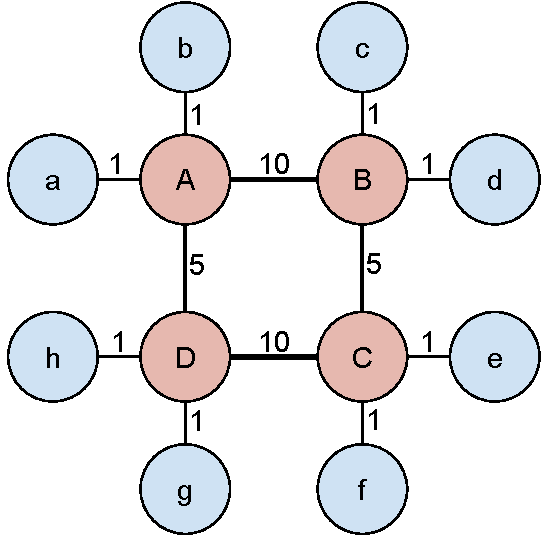
\includegraphics[width=0.8\linewidth]{images/estrutura_abst_topo.pdf}
    \caption{Topologia.}
    \label{fig:estru:topo}
\end{subfigure}
\begin{subfigure}{.5\textwidth}
    \centering
    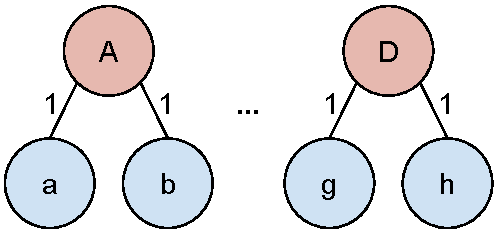
\includegraphics[width=0.8\linewidth]{images/estrutura_abst_arvore.pdf}
    \caption{Árvore.}
    \label{fig:estru:arvore}
\end{subfigure}
\begin{subfigure}{.5\textwidth}
    \centering
    \begin{tabular}{|l|c|c|c|c|c|c|c|c|}
        \cline{1-6}
        Índice     & 0 & 2  & 4 & 6 & 8  \\ \hline
        Linha      & B & D & A & C & B & D & A & C  \\ \hline
        Distância  & 10 & 5 & 10 & 5 & 5 & 10 & 5 & 10 \\ \hline
    \end{tabular}
    \caption{CSC.}
    \label{fig:estru:csc}
\end{subfigure}
\begin{subfigure}{.5\textwidth}
    \centering
    \begin{tabular}{|c|c|c|c|c|}
        \hline
         M & A & B  & C & D  \\ \hline
         A & X & 10 &   & 5  \\ \hline
         B & X & X  & 5 & 15 \\ \hline
         C & X & X  & X & 10  \\ \hline
         D & X & X  & X & X  \\ \hline
    \end{tabular}
    \caption{Matriz.}
    \label{fig:estru:matriz}
\end{subfigure}
\caption[Representação das estruturas utilizadas.]{Representação da topologia mostrada em (a)-(b) de acordo com as estruturas propostas.}
\label{fig:estru}
\end{figure}

A Figura~\ref{fig:estru} apresenta as estruturas propostas para representar a topologia da Figura~\ref{fig:estru:topo}, os PEs então em azul, as máquinas em vermelho e os números nas conexões representam uma latência. 
A Figura~\ref{fig:estru:arvore} apresenta a estrutura hierárquica de árvore de duas das máquinas desta topologia e a Tabela~\ref{fig:estru:csc} a representação das distâncias das máquinas com CSC. 
A estrutura matricial para memoização das distâncias entre máquinas é representada pela Tabela~\ref{fig:estru:matriz}. Ela utiliza uma estrutura matricial proposta para a memoização de distâncias entre as máquinas, onde a primeira linha e primeira coluna indicam uma máquina e as células internas representam as distâncias.
Um 'X' indica que a posição não é armazenada para economia de memória e um espaço em branco indica uma distância ainda não calculada mas com memória alocada.

Nesta estrutura, a complexidade de acesso de uma distância qualquer é de $O(g)$ e de $O(1)$ caso tenha sido calculada anteriormente.
Sendo $c$ a média do número de PEs por máquinas e $m$ o número de máquinas, o uso de memória é de $O(mc)$ para as estruturas de árvore, de $O(\frac{p+l}{c})$ para o CSC e de $O(\frac{p^2}{2c^2})$ para a matriz de memoização.
O custo de criação e inicialização da estrutura é dependente do número de PEs na rede e do tempo de acesso e descobrimento das informações topológicas usadas de base, como a do \hwloc ou do \textit{runtime} \charm.



\section{Funcionalidades}
\label{sec:func}

A interface da Net Topo contém métodos para obter informações da topologia, cálculo de distância, \hops e proximidade, abordados na Seção~\ref{sec:distances}, e para a serialização das estruturas em um arquivo XML, descrito na Seção~\ref{sec:xml}.
Na Seção~\ref{sec:init} é detalhado como são inicializadas as estruturas da abstração.
A Tabela~\ref{tab:topo_infos} apresenta as informações de topologia disponíveis na abstração, seus métodos e suas assinaturas.
A palavra ``nó'' é utilizada para representar um agrupamento interno de PEs de uma máquina, realizado por nível de \textit{cache} compartilhada.

\setlength{\tabcolsep}{0.5em}
\begin{table}[t]
    \centering
    \begin{tabular}{l c l}
        \toprule
        \textbf{Método} &    \textbf{Entrada} &    \textbf{Saída} \\ \midrule
        \textit{num\_pes} &    - &    Número de PEs na topologia   \\ 
        \textit{num\_machines} &    - &    Número de máquinas na topologia   \\
        \textit{num\_nodes} &    - &    Número de nós na topologia   \\
        \textit{machine\_of} & um PE & Máquina onde o PE se encontra  \\
        \textit{node\_of} & um PE & Nó onde o PE se encontra  \\
        \textit{pes\_of\_machine} &  uma máquina & Uma lista dos PEs da máquina \\
        \textit{on\_same\_machine} &  uma PE & Uma lista dos PEs na mesma máquina \\
        \textit{pes\_of\_node} &  um nó & Uma lista dos PEs do nó \\
        \textit{on\_same\_node} &  uma PE & Uma lista dos PEs no mesmo nó \\
        \textit{net\_neighbors} &  uma máquina & Uma lista de máquinas vizinhas \\ \textit{num\_net\_links} & - & Número de \textit{links} na rede \\
        \textit{fill\_memoi} & - & Preenche a matriz de memoização \\
        \bottomrule
    \end{tabular}
    \caption[Métodos de informação de topologia.]{Métodos de informação de topologia. A primeira coluna apresenta a assinatura do método. A coluna Entrada apresenta as informações requeridas pelo método e a coluna Saída indica o que o método retorna.}
    \label{tab:topo_infos}
\end{table}

\subsection{Funções de Distância e Proximidade}
\label{sec:distances}

Métricas de proximidade entre dois PEs e a distância entre eles são relevantes para realizar uma alocação de tarefas eficiente e que leve em consideração a topologia de rede utilizada.
Três métricas de distância foram implementadas dentro da Net Topo: uma função de proximidade, um cálculo de \hops e um cálculo de distância mínima.

Como os custos de comunicação aumentam conforme a distância entre PEs, saber em que nível a comunicação irá acontecer permite uma estimativa do custo de comunicação entre dois PEs.
Para determinar qual a camada de comunicação entre dois PEs, basta saber da topologia de máquina de uma delas. 
Se não estiverem na mesma máquina, esta acontecerá em rede. 
Se estiverem, é possível determinar em qual nível.
A função de proximidade realiza um cálculo simples para indicar o quão próximo um PE está de outro na topologia de máquina.
O método que implementa esta função tem o nome de \textit{proximity}, recebe dois identificadores de PE como entrada e retorna um inteiro de acordo com a função de proximidade descrita na Tabela~\ref{tab:proximity}.
Saber o quão próximo um ponto está de outro em uma rede é dependente ou de sua distância mínima ou da quantidade de \hops até ele, que caem no escopo das próximas funções e não são tão simples.


% tabelinha de retorno de função de proximidade
\setlength{\tabcolsep}{0.5em}
\begin{table}[!ht]
    \centering
    \begin{tabular}{c l}
        \toprule
        \textbf{Saída} &    \textbf{Relação entre os dois PEs} \\ \midrule
        3 & São o mesmo.   \\ %\hline
        2 & Estão na mesma máquina e no mesmo nó.   \\ %\hline
        1 & Estão na mesma máquina mas não no mesmo nó.   \\ %\hline
        0 & Não estão na mesma máquina. \\ \bottomrule
    \end{tabular}
    \caption[Função de proximidade]{Função de proximidade entre dois PEs. A primeira coluna representa a saída da função e a segunda a relação entre os dois PEs.}
    \label{tab:proximity}
\end{table}

Um cálculo de \hops permite observar a proximidade entre dois PEs em uma rede, a quantidade de \links utilizada em uma comunicação entre os dois e ter uma noção de distância sem precisar obter as latências da rede.
O cálculo de \hops é implementado pelo método \textit{hop\_count}, que recebe identificadores de dois PEs, um origem e um destino, e retorna um inteiro com o número de \hops.
A implementação é uma busca em largura pela estrutura CSC, iniciando no PE origem e contando o número de expansões até alcançar o PE destino.
Esta implementação não utiliza o mecanismo de memoização, pois as distâncias mínimas são diferentes do número de \hops.


Um cálculo de latência mínima entre dois PEs permite considerar com precisão a latência de comunicação entre eles mas não oferece uma perspectiva de contenção.
Essa informação é útil para um escalonador ou balanceador que visa reduzir as latências de comunicação do sistema.

O cálculo de distância mínima foi implementando utilizando o algoritmo de Djisktra modificado para incluir o mecanismo de memoização.
Antes de ser executado na camada de rede, é obtida a máquina dos dois PEs e é verificado se são os mesmos. Caso sejam, é retornado $0.1$ se estão no mesmo nó, $0$ se são o mesmo PE e $0.2$ caso nenhum dos dois seja verdade.

O Algoritmo~\ref{alg:dists} apresenta o algoritmo modificado.
$M$ é uma função cujo domínio são dois PEs da topologia, $x$ e $y$, e a imagem é a distância entre eles seguindo uma matriz de distâncias. %ref equação
%A função $M$ é uma função de mapeamento $M:x,y \rightarrow \mathbb{Z} \mid x, y \in \mathbb{Z}$, onde $x$ e $y$ representem máquinas e o valor retornado representa a distância entre eles.
A função representa o mecanismo de memoização implementado com uma matriz triangular superior.
Para inserir um valor na posição $(x, y)$ da matriz de distâncias de $M$, se utiliza a notação $M[x][y] \leftarrow$ distância.
O mapeamento $D:m \rightarrow d$ associa uma máquina $m$ a uma distância $d$ da origem.
A notação $D(m) \rightarrow d$ é utilizada para indicar que uma nova associação foi criada.

No inicio do Algoritmo~\ref{alg:dists} é verificado se a distância entre a origem e o destino já não é conhecida na estrutura de memoização.
Caso seja, a distância é retornada e o algoritmo encerra.
Nas linhas 1 a 10 ocorre a inicialização do algoritmo, adicionando máquinas cuja distância já se sabe ao conjunto das não visitadas. 
Nas linhas 11 a 27 é executado o laço principal, onde, para cada máquina do conjunto de máquinas não visitadas ($U$), se alcança suas vizinhas e, caso não tenham sido alcançadas, as adiciona em $U$.
Caso a máquina vizinha tenha sido alcançada, é verificado se a distância atual até ela não é menor do que a armazenada no momento (linha 18).
Antes de trocar a máquina sendo visitada (linhas 20 a 22), se insere sua distância em $M$ para uso futuro, a adiciona ao conjunto das visitadas ($V$) e a retira de $U$.
Ao se trocar de máquina (linha 23) é sempre escolhida a máquina menos distante de $U$ e, caso seja o destino, sua distância é adicionada em $M$ e o algoritmo termina retornando a distância encontrada.
Caso não se alcance o destino, é retornado $-1$.

\begin{algorithm}[t]
\caption{Djisktra Modificado}
\label{alg:dists}
    \DontPrintSemicolon
    \SetKwInOut{Estrutura} {Estruturas}
    \Entrada{origem: máquina de origem, destino: máquina destino}
    \Saida{Distância entre a origem e o destino}
    \Estrutura{$V$: Conjunto de máquinas visitadas, \\ 
                $U$: Conjunto de máquinas não visitadas, \\
                $D$: Mapeamento de uma máquina para uma distância.}
                \BlankLine
    $U \leftarrow \{$origem$\}$\;
    $D($origem$) \leftarrow {0}$\;
     \ForEach{máquina "x" da topologia}{
        $U \leftarrow U \cup \{x\}$\;
        \eIf{$M[$origem$][x]$ existe}
            {$D(x) \rightarrow M[$origem$][x]$}
        {$D(x) \rightarrow \infty$}
    }
    atual $\leftarrow$ origem  \tcp*{máquina sendo iterada}
    dist $\leftarrow 0$  \tcp*{distância até o atual}
    \While{$U \neq $\O}{
        \ForEach{máquina "v" $\mid$ v é vizinha da máquina atual}{
            $dist\_v \leftarrow$ dist $+$ distância entre atual e $v$\;
            \eIf{$v \notin \{V \cup U\} $}{
                $U \leftarrow U \cup \{v\}$\;
                $D(v) \rightarrow dist\_v$}
                {\If{$v \in U$ e $D(v) > dist\_v$}
                    {$D(v) \rightarrow dist\_v$}
            }
        }
        $M[$origem$][$ atual$] \leftarrow$ dist\;
        $V \leftarrow V \cup \{$atual$\}$\;
        $U \leftarrow U \setminus \{$atual$\}$\;
        atual $\leftarrow x \mid x \in U$ e tenha a menor distância em $U$\;
        dist $\leftarrow D($atual$)$\;
        \If{atual = destino}{
            $M[$origem$][$ destino$] \leftarrow$ dist\;
            retorna dist}
    }
    retorna $-1$ \tcp*{não alcançou o destino}
\end{algorithm}

Foi cogitado a importação das distâncias memoizadas de uma máquina vizinha na linha 12 com um laço adicional, mas geraria um sobrecusto que não seria sempre útil.
A utilização dela não é sempre melhor devido ao fato de que a distância memoizada é relativa à distância de alcançar a máquina sendo visitada, portanto não necessariamente será o menor até o alvo, mas somente a menor a partir do atual.


\subsection{Serialização}
\label{sec:xml}

O armazenamento da estrutura de topologia permite utilizar a mesma estrutura topológica em execuções diferentes, reduzindo o custo de inicialização da abstração e mantendo persistência das informações de custos já calculadas.

Para realizar a serialização das estruturas da Net Topo, foi utilizado a biblioteca de serialização \textit{Cereal} ~\cite{website:Cereal}. 
A biblioteca foi escolhida pela sua simplicidade, velocidade e pela compatibilidade com a linguagem \textit{C++}.
O arquivo de serialização gerado está na linguagem XML (\textit{Extensible Markup Language}), o mesmo utilizada pelo \hwloc, pois oferece legibilidade do que está armazenado.

Foram criadas as funções \textit{save\_topology} e \textit{load\_topology} para exportar e importar, respectivamente, um arquivo XML com nome passado por parâmetro.
Caso nenhum nome seja passado, o nome padrão utilizado é ``\textit{net\_topo.xml}''.
Para inicializar as estruturas com as informações armazenadas num arquivo, basta chamar a função \textit{load\_topology} após a criação de uma instância da Net Topo.


\subsection{Inicialização}
\label{sec:init}

Para ampliar e facilitar seu uso, a Net topo é uma abstração desacoplada de outras implementações, o que faz que sua inicialização seja dependente de alguma fonte de informações topológicas.
As informações de rede podem ser obtidas manualmente ou através de mecanismos automáticos, como o \netloc.
O \textit{runtime} \charm obtém informações de topologia automaticamente.
A Seção~\ref{sec:init:charm} apresenta detalhes das informações obtidas pelo \charm e como estas informações são passadas para a abstração.

Neste trabalho foram criadas três inicializações: uma manual, que recebe uma entrada padrão; uma automática, utilizando um adaptador para o \charm; e uma através de um arquivo XML gerado anteriormente pelo Net Topo.
As três formas de inicialização são abordadas a seguir e todas têm a opção de remover o mecanismo de memoização.

\subsubsection{Inicialização Manual}

Um padrão de entrada com as informações de topologia necessárias foi criado para a função de inicialização do Net Topo.
O algoritmo de funcionamento da inicialização da estrutura foi dividido em dois e é descrito pelos Algoritmos~\ref{alg:init_machine} e \ref{alg:init_network}. 


A inicialização da topologia de máquina é descrita pelo Algoritmo~\ref{alg:init_machine} e deve ser executada antes, por capturar informações necessárias para a divisão de rede.
O objetivo deste algoritmo é criar um mapeamento entre PEs, nós e máquinas, para a representação da topologia de máquina.
O algoritmo necessita como entrada um conjunto de triplas $(pe, m, n) \mid pe, m, n \in \mathbb{Z}$ onde $pe$ representa um PE, $m$ representa a máquina deste PE e $n$ o seu nó. 
Os nós recebidos na entrada são relativos a uma máquina e não ao sistema como um todo.
O algoritmo assume que todos os PEs de uma máquina estejam em sequência nesta lista.
O resultado deste algoritmo são duas listas de duplas $PM$ e $PN$, um agrupamento de PEs por nó e um agrupamento de PEs por máquina.
O mapeamento $MP:m\rightarrow P$ associa um conjunto de PEs $P$ a máquina $m$.
Para associar o conjunto $P$ a uma máquina $m$ no mapeamento $MP$, é usada a notação $MP(m) \rightarrow P$.
O mapeamento $NP:n\rightarrow P$ associa um conjunto de PEs $P$ a um nó $n$.
Para adicionar um PE $pe$ ao conjunto $P$ de um nó $n$, é utilizado a notação $NP(m) \rightarrow pe$.
A notação $\mid NP \mid$ é utilizada para indicar o número de mapeamentos em $NP$.

\begin{algorithm}[t]
    \DontPrintSemicolon
    \SetKwInOut{Estrutura}{Estruturas}
    \Entrada{$T$: Conjunto ordenado de triplas $(m, pe, n)$, onde $m$ é uma máquina, $pe$ um PE desta máquina e $n$ o nó deste PE.}
    \Saida{ $PM$: Conjunto de duplas $(pe, m)$ onde $pe$ é um PE e $m$ sua máquina, \\
            \hspace{12mm} $PN$: Conjunto de duplas $(pe, n)$ onde $pe$ é um PE e $n$ seu nó, \\
            \hspace{12mm} $MP$: Mapeamento de cada máquina ao seu conjunto de PEs, \\
            \hspace{12mm} $NP$: Mapeamento de cada nó aos seus PEs.}
    \Estrutura{$P$: Conjunto de PEs de uma máquina.}

    \BlankLine
    $maq \leftarrow 0$, \xspace 
    $no \leftarrow 0$ \tcp*{máquina e nó sendo iterados}
    $n\_nos \leftarrow 0$\;
    $P \leftarrow $\O, \xspace
    $PM \leftarrow $\O, \xspace
    $PN \leftarrow $\O\;
    \ForEach{ tripla (m, pe, n) em T}{
        $PM \leftarrow PM \cup \{(pe, m)\}$\;
        \If{m $\neq$ maq}{
            $MP(maq) \rightarrow P$\;
            $maq \leftarrow m$\;
            $n\_nos \leftarrow \mid NP \mid$ \;
            $P \leftarrow $\O\;
        }
        $no \leftarrow n + n\_nos$\;
        $PN \leftarrow PN \cup \{(pe, no)\}$\; 
        $NP(no) \rightarrow pe$\;
        $P \leftarrow P \cup \{pe\}$\;
    }
    $MP(maq) \rightarrow P$\;
    
\caption{Inicialização da Topologia de Máquina}
\label{alg:init_machine}
\end{algorithm}

Nas linhas 1 e 3 do Algoritmo~\ref{alg:init_machine} são feitos os ajustes iniciais para a execução. 
O laço principal (linhas 4 a 15) mapeia cada PE para a sua máquina e para o seu nó (com os conjuntos $PM$ e $PN$). 
Cada máquina e cada nó é associado a um conjunto de PEs com os mapeamentos $MP$ e $NP$, respectivamente.
Na linha 11 é re-identificado o nó do PE, para ser absoluto e não relativo à máquina que estava.
Quando se troca a máquina sendo iterada (linhas 6 a 10) são agrupados para a máquina todos os PEs em $P$ para utilizar no mapeamento $MP$.
Na troca de máquina também é atualizada a contagem de nós encontrados até o momento, para modificar o número de identificação dos nós.



\begin{algorithm}[t]
    \DontPrintSemicolon
    \SetKwInOut{Estrutura}{Estruturas}
    \Entrada{$T$: um conjunto de triplas $(pe, v, d)$, onde $pe$ e $v$ são PEs vizinhos e $d$ a distância entre eles.}
    \Saida{$G$: um grafo de máquinas que representa a topologia de rede.}
    \Estrutura{
                $D$: conjunto de duplas \{$v, d$\}, onde $v$ é uma máquina e $d$ uma distância.
    }
    \BlankLine
    $V \leftarrow$ \O, \xspace
    $E \leftarrow$ \O\;
    \ForEach{máquina m na topologia}
        {$D \leftarrow vizinhas(m, T)$\;
        $V \leftarrow V \cup \{m\}$\;
        \ForEach{ dupla (v, d) em D} 
            {$V \leftarrow V \cup \{v\}$ \;
             $E \leftarrow E \cup \{(m, v)\}$\;
             $W(m, v) \rightarrow d$}
    }

\caption{Inicialização da Topologia de Rede}
\label{alg:init_network}
\end{algorithm}

O algoritmo de inicialização de topologia de rede, Algoritmo~\ref{alg:init_network}, captura as informações de vizinhança descrita por uma entrada ($T$), estabelece as vizinhanças em nível de máquina e as armazena em um grafo $G$.
O grafo $G$ é um grafo representando uma topologia de rede e é dado por $G = (V, E, W) \mid V = \{$ união dos $v$, que representa máquinas$\}$, $E = \{$ união das relações $(v, u) \mid v, u \in V\}$, $W$ é uma função de peso $W:v,u \rightarrow w$.
Este grafo é implementado com um CSC.
A função $vizinhas$ utilizada é descrita pelo Algoritmo~\ref{alg:vizinhos} e encontra as máquinas vizinhas de uma determinada máquina e suas distâncias até ela.

O algoritmo de inicialização da topologia de rede busca todas as máquinas vizinhas de cada máquina na topologia (linha 3).
Esta máquina é adicionada ao grafo como um vértice (linha 4) e para cada máquina vizinha é criado uma aresta com peso equivalente a distância até ela (linhas 7 e 8).

\begin{algorithm}
    \DontPrintSemicolon
    \SetKwInOut{Estrutura}{Estruturas}
    \Entrada{$T$: um conjunto de triplas $(pe, v, d)$, onde $pe$ e $v$ são PEs vizinhos e $d$ a distância entre eles, \\
            \hspace{15mm} $m$: uma máquina cuja vizinhança se quer conhecer.}
    \Saida{$V$: conjunto de duplas \{$v, d$\}, onde $v$ é uma máquina vizinha a $m$ e $d$ a distância entre elas.
                }
    \BlankLine
    
    $maq\_v \leftarrow 0$\; 
    $V \leftarrow $\O\;
    \ForEach{ tripla (pe, v, d) em T $\mid$ maquina\_de(pe) = m}{
        $maq\_v \leftarrow maquina\_de(v)$\;
        \eIf{maq\_v $\notin$ V}
            {$V \leftarrow V \cup \{maq\_v, d\}$}
            {\If{$V(maq\_v) > d$}
                {$V(maq\_v) \leftarrow d$}
        }
    }
    $V \leftarrow V \setminus \{m\}$\;
\caption{Máquinas Vizinhas}
\label{alg:vizinhos}
\end{algorithm}

O Algoritmo~\ref{alg:vizinhos} estabelece um conjunto das máquinas vizinhas de $m$ e a distância entre elas.
A funcionalidade $maquina\_de(pe)$ retorna a máquina de um PE $pe$.
O laço principal do algoritmo obtém todos os vizinhos de cada PE da máquina, criando duplas de máquinas vizinhas com as suas distâncias, agregadas no conjunto $V$.
Como cada máquina tem vizinhança consigo mesma, é necessário retirar ela mesma do mapeamento (linha 10).
Para obter a distância de uma máquina a outra, a menor distância dentre os PEs é utilizada, assumindo que uma latência entre PEs da mesma máquina possa ser desconsiderada no cálculo.

\subsubsection{Inicialização via XML}

A inicialização XML importa informações salvas anteriormente em um arquivo XML, restaurando a topologia armazenada e sua matriz de distâncias.
Para utilizar esta inicialização basta invocar o método \textit{load\_topology}, descrito na Seção ~\ref{sec:xml}.
A utilidade desta inicialização se dá pela remoção do tempo de descobrimento da topologia e pela importação da matriz de distâncias utilizada em execuções anteriores.
Esta inicialização só pode ocorrer se houver um arquivo XML de topologia salvo anteriormente.

% ver diferença de importação e descobrimento em testes de overhead?

\subsubsection{\charm}
\label{sec:init:charm}
A inicialização através do \textit{runtime} do \charm é automática mas apresenta uma série de limitações devido a incompletude das informações coletadas pelo \textit{runtime} e pelo armazenamento destas, abordadas adiante.

O \charm possui duas maneiras de descobrir uma topologia: de maneira manual, com opções de execução, da classe \textit{TopoManager} e topologias fixas como \textit{Cray} e \textit{BlueGene}; e de maneira automática, através de envio de mensagens entre os PEs utilizados e enquadramento da topologia encontrada em um dos tipos pré-estabelecidos em sua classe \textit{topology}, como \textit{Mesh} 2D, \textit{Torus} ou \Fatt. 
A escolha destas abordagens se deve a otimizar o calculo de \hops, que depende só das posições da origem e do destino nestas topologias, evitando um algoritmo com travessia de grafo.
Porém, os únicos métodos obrigatórios em cada topologia são os de encontrar o número máximo de vizinhos e os seus vizinhos, o que acarreta em dificuldades para algoritmos que consideram topologias genéricas.

A obtenção de topologia do \charm inclui três problemas que não eram esperadas no inicio deste trabalho:
(i) não há armazenamento de latência de mensagens entre PEs reconhecidos na topologia; (ii) não há informações sobre compartilhamento de \textit{cache} entre PEs; e (iii) há imprecisões em certas funções quando as máquinas da rede não são iguais.
A ausência de latências impossibilita cálculos de distância que não sejam através de \hops, pois não há nenhuma outra métrica.
A falta de informações sobre compartilhamento de \textit{cache} impede o agrupamento de PEs por grupos de \textit{cache} e um detalhamento de cada máquina na topologia.
As funções imprecisas são relacionadas ao número de PEs por nó físico da topologia, que são distribuídos igualmente pelo número de máquinas na rede.
Esse agrupamento equivalente impossibilita saber quais PEs estão efetivamente em quais máquinas, gerando informações imprecisas para a secção entre topologia das máquinas e topologia da rede.

A Figura~\ref{fig:charm_imprecision} apresenta uma comparação entre uma topologia real com máquinas heterogêneas e a sua representação dentro do sistema do \charm. A topologia é composta por duas máquinas, uma com 4 cores, sem agrupamento de \textit{cache}, e a segunda com 8 cores e 4 agrupamentos de \textit{cache}.

\begin{figure}[h]
\begin{subfigure}{.55\textwidth}
    \centering
    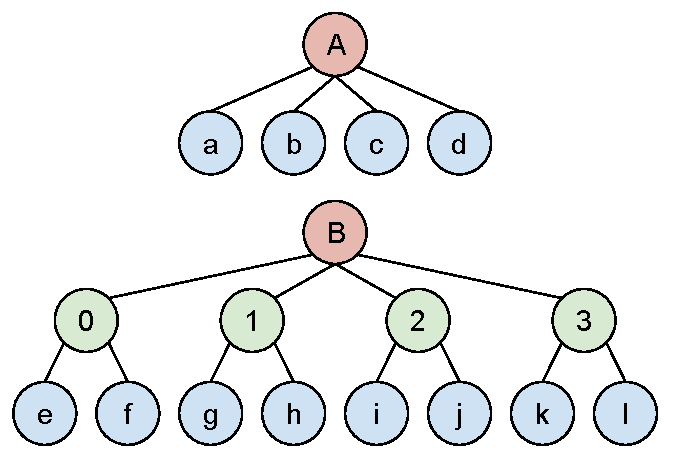
\includegraphics[width=0.85\linewidth]{images/init_real_topo.pdf}
    \caption{Topologia Real}
    \label{fig:charm_imprecision:real}
\end{subfigure}
\begin{subfigure}{.45\textwidth}
    \centering
    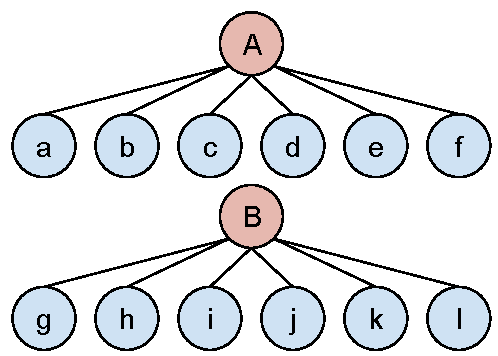
\includegraphics[width=0.8\linewidth]{images/init_charm_topo.pdf}
    \caption{Agrupamento realizado pelo \charm}
    \label{fig:charm_imprecision:charm}
\end{subfigure}
\caption[Comparação entre a topologia real e a encontrada pelo \charm.]{Comparação entre a topologia real (esquerda) e a encontrada pelo \charm (direita). Máquinas em vermelho e letras maiúsculas, agrupamentos de \textit{cache} em verde e numerais, e PEs em azul e letras minúsculas.}
\label{fig:charm_imprecision}
\end{figure}

Para interagir com o \textit{runtime} do \charm e extrair as informações topológicas foi criado um adaptador de nome \textit{net\_topo\_charm\_proxy}.
Dentro do adaptador foram criados duas inicializações intermediárias: \textit{init} e \textit{init\_no\_nodes}.
O primeiro extrai os agrupamentos de máquinas enquanto o segundo ignora a parte de topologia de máquina do \charm e trata cada PE como uma máquina individual.
Portanto, o segundo mantém a precisão das conexões mas perde qualquer informação relacionada ao agrupamento de PEs em máquinas.
Ambas as inicializações utilizam o padrão de inicialização da Net Topo.



% detalhamento da entrada para uma inicialização, algoritmo
